
% This LaTeX was auto-generated from MATLAB code.
% To make changes, update the MATLAB code and republish this document.

\documentclass{article}
\usepackage{graphicx}
\usepackage{color}

\sloppy
\definecolor{lightgray}{gray}{0.5}
\setlength{\parindent}{0pt}

\begin{document}

    
    
\subsection*{Contents}

\begin{itemize}
\setlength{\itemsep}{-1ex}
   \item Load in the coordinates of vectors representing points on our "potato"
   \item EXAMPLE of applying a transformation to the potato's points
   \item YOUR ANSWERS
\end{itemize}
\begin{verbatim}
% Computational Linear Algebra (EK 103), Spring 2025, Boston University
% Problem Set 7, Problem 1(d), plotting transformations of a potato
% March 2025

% Set up the workspace
clear all; close all; clc;
\end{verbatim}


\subsection*{Load in the coordinates of vectors representing points on our "potato"}

\begin{verbatim}
coord_filename = "potato_points.csv";
try
    pts = readmatrix(coord_filename);
catch anyerror
    disp("ERROR! Couldn't find potato_points.csv. Is it in the same directory as ps7_problem1d.m ?? Check the homework instructions!");
    return
end
\end{verbatim}


\subsection*{EXAMPLE of applying a transformation to the potato's points}

\begin{verbatim}
% the identity matrix should keep the potato where it is
I = [1, 0;
     0, 1];
pts_example = I*pts;

% This is just to check you've got the right files here, no need for more
% of the "try catch" stuff more than once.
try
    plot_potatoes(pts, pts_example, "Identity Matrix");
catch anyerr
    disp("Error! Couldn't find the function that plots our potato points. Is plot_potatoes.m in the same directory as ps7_problem1d.m ??")
    return
end
\end{verbatim}

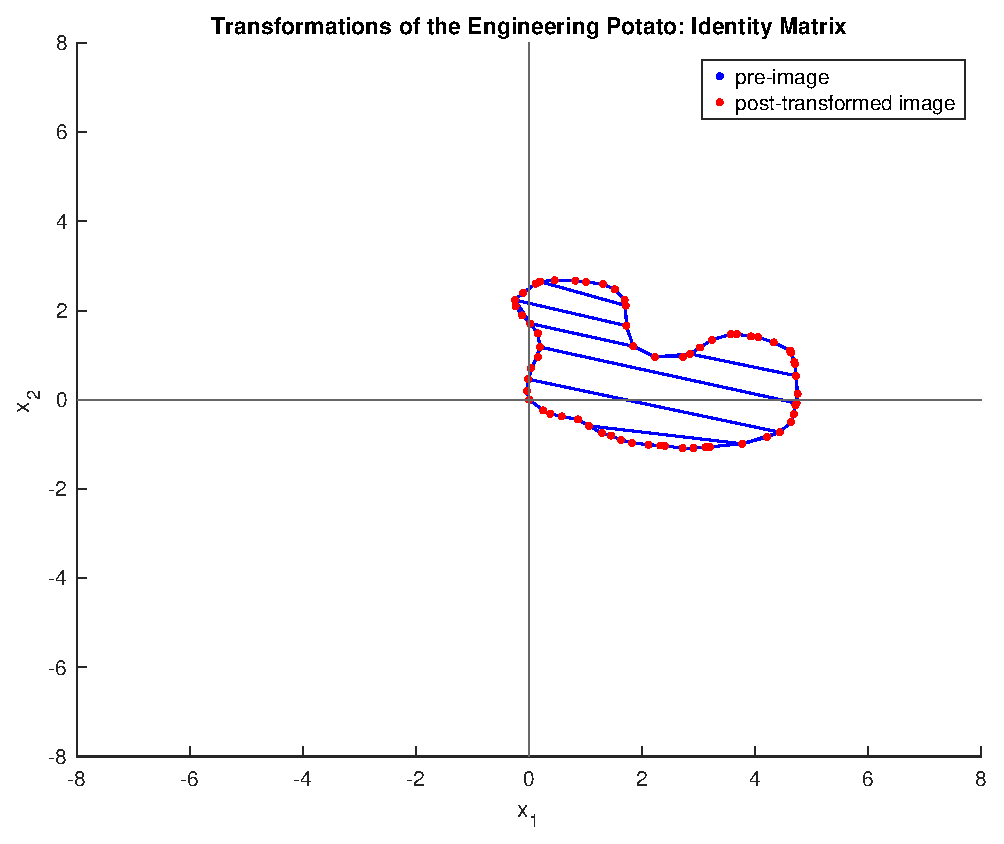
\includegraphics [width=4in]{ps7_problem1d_01.eps}


\subsection*{YOUR ANSWERS}

\begin{verbatim}
% 1(c) (i)
A1 = [0,1;1,0]
pts1 = A1*pts;
plot_potatoes(pts, pts1, "A1");

% 1(c) (ii)
A2 = [1,0;0,2]
pts2 = A2*pts;
plot_potatoes(pts, pts2, "A2");

% 1(c) (iii)
A3 = [1,0;-0.5,1]
pts3 = A3*pts;
plot_potatoes(pts, pts3, "A3");

% 1(c) (iv)
A4 = [1,0;0,0]
pts4 = A4*pts;
plot_potatoes(pts, pts4, "A4");

% 1(c) (v)
% Note for those new to matlab: sqrt(x) gives you the square root of x.
A5 = [0.5, (-sqrt(3))/2;(sqrt(3))/2, 0.5]
pts5 = A5*pts;
plot_potatoes(pts, pts5, "A5");
\end{verbatim}

        \color{lightgray} \begin{verbatim}
A1 =

     0     1
     1     0


A2 =

     1     0
     0     2


A3 =

    1.0000         0
   -0.5000    1.0000


A4 =

     1     0
     0     0


A5 =

    0.5000   -0.8660
    0.8660    0.5000

\end{verbatim} \color{black}
    
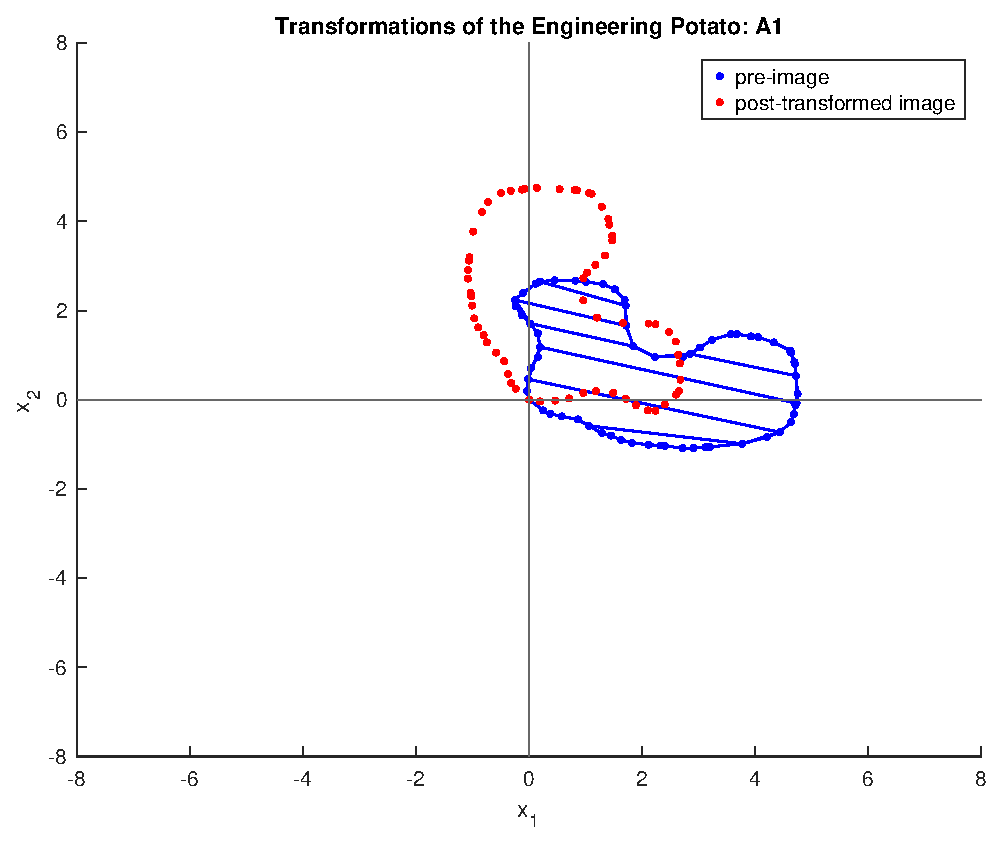
\includegraphics [width=4in]{ps7_problem1d_02.eps}

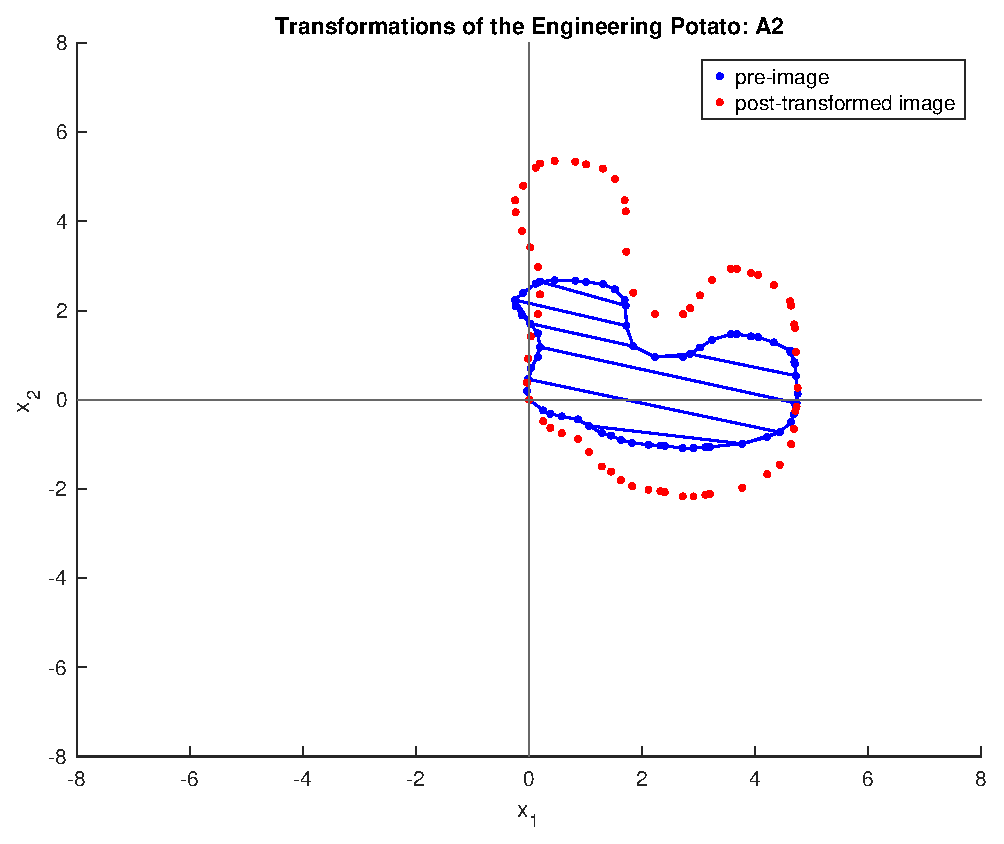
\includegraphics [width=4in]{ps7_problem1d_03.eps}

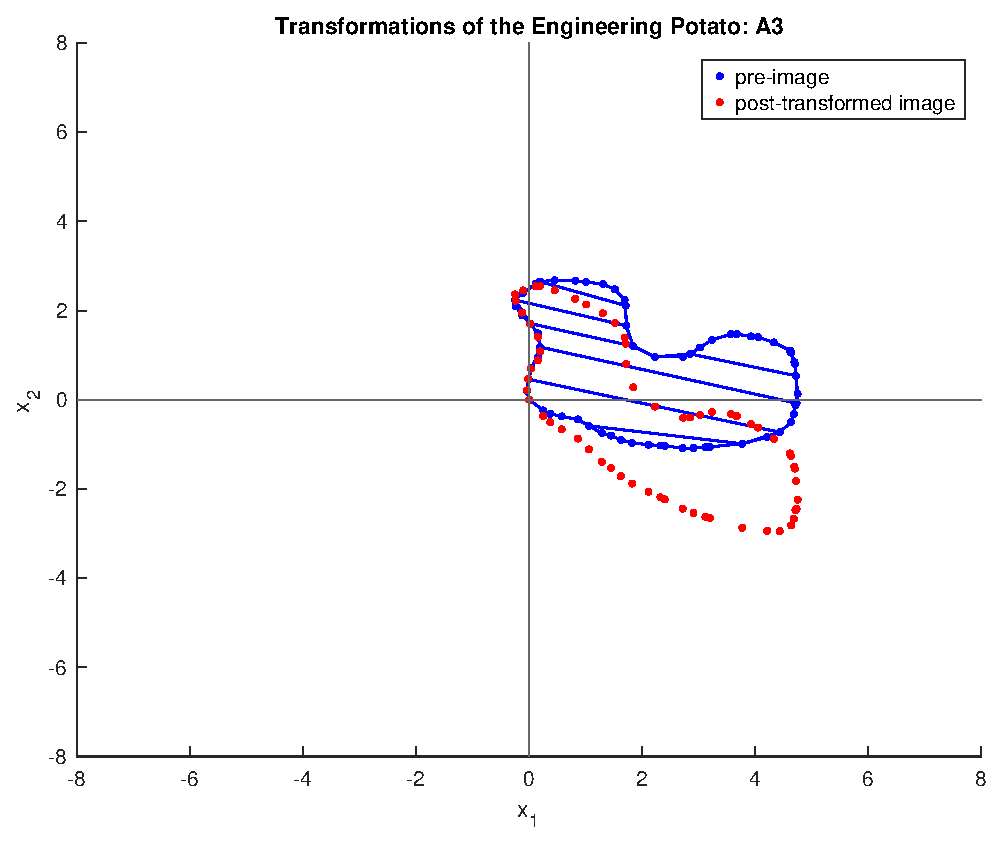
\includegraphics [width=4in]{ps7_problem1d_04.eps}

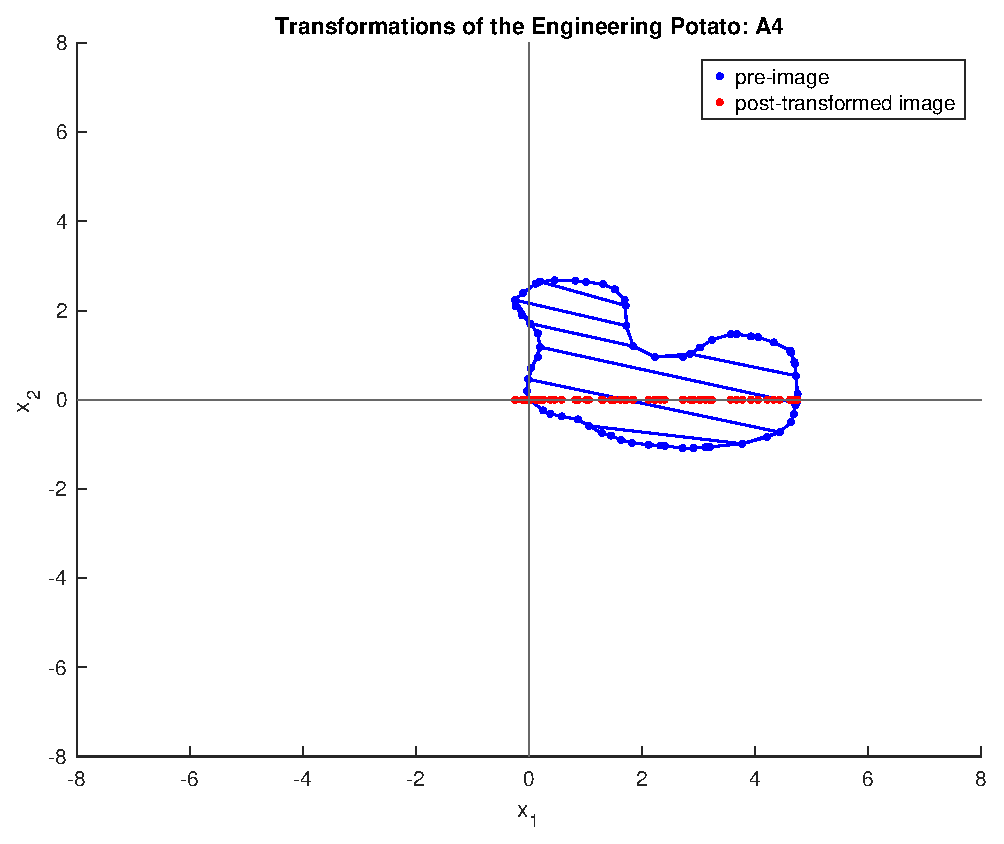
\includegraphics [width=4in]{ps7_problem1d_05.eps}

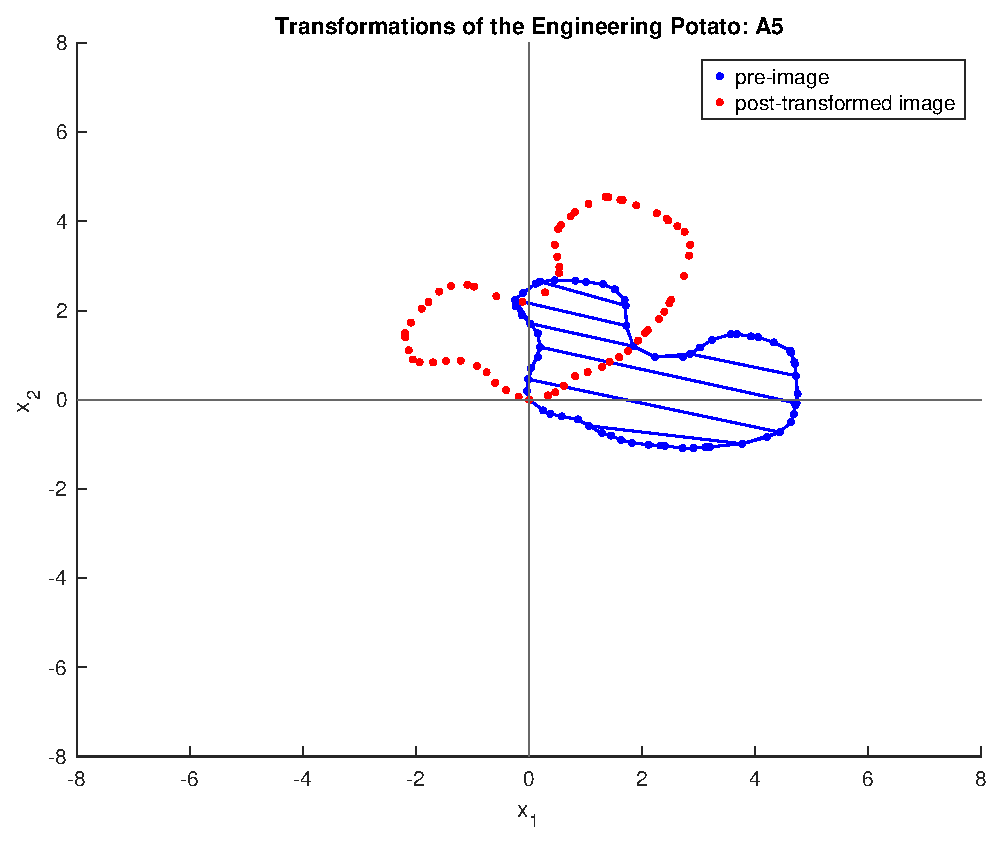
\includegraphics [width=4in]{ps7_problem1d_06.eps}



\end{document}

